\documentclass[tikz,border=2,dvspsnames]{standalone}
\usetikzlibrary{shadows,arrows,arrows.meta,shapes,positioning,calc,backgrounds,fit}
\newcommand{\vanish}[1]{}
% Define the layers to draw the diagram
%
\begin{document}
%
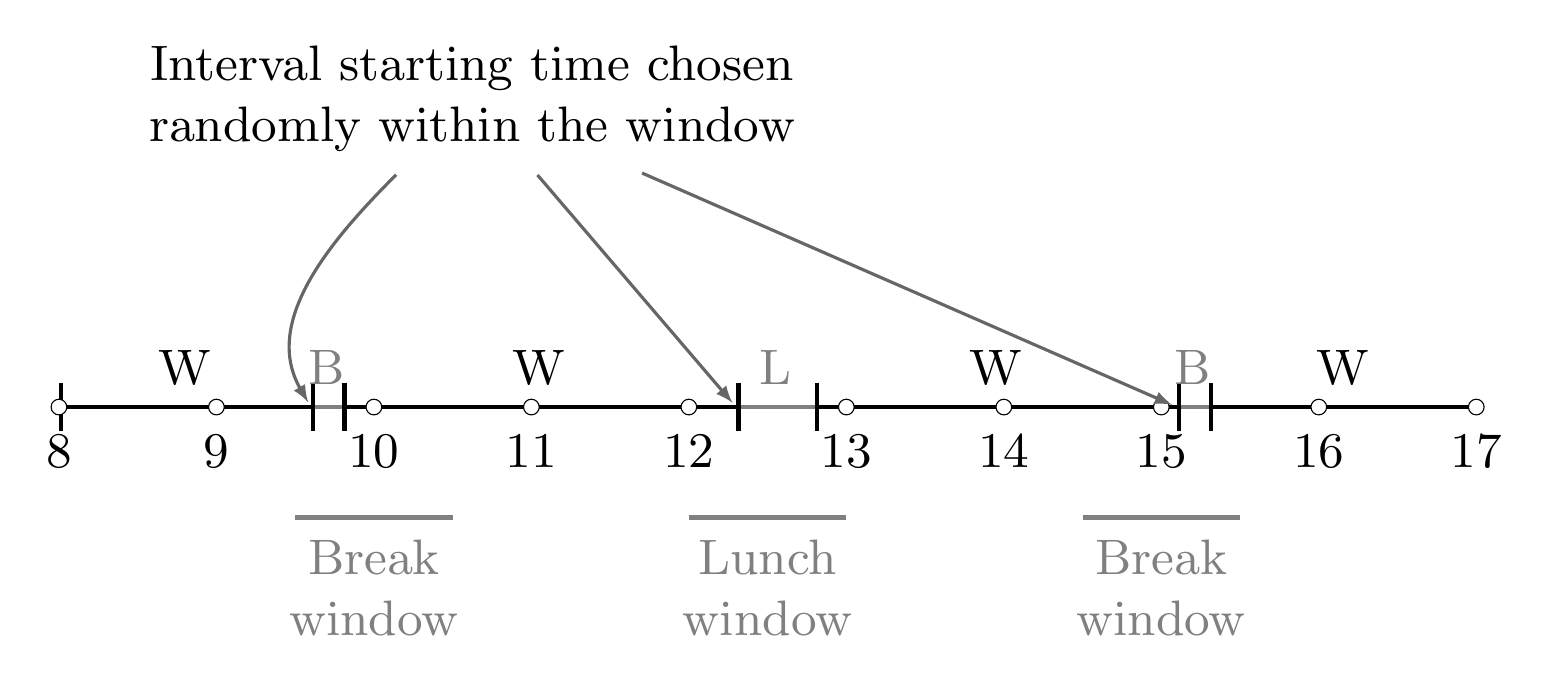
\begin{tikzpicture}
[scale=2,node distance=1cm, transform shape,font=\small,
edge/.style={black!60,>=latex, shorten >=2pt, shorten <=2pt, line width=.4mm},
tic/.style={circle,inner sep=1pt,draw,fill=white}]
%%%%%%%%%%

\def \window {1}
\def \breakInterval {.2}
\def \lunchInterval {.5}

\draw[ultra thick,{|[width=6mm]}-] (8,0) to node[midway,above] {W} (9.6,0);
\draw[ultra thick,{|[width=6mm,black]}-,black!50] (9.6,0) -- node[midway,above] {B} +(\breakInterval,0);
\draw[ultra thick,{|[width=6mm,black]}-] (9.6+\breakInterval,0) to node[midway,above] {W} (12.3,0);
\draw[ultra thick,{|[width=6mm,black]}-,black!50] (12.3,0) to node[midway,above] {L} +(\lunchInterval,0);
\draw[ultra thick,{|[width=6mm,black]}-] (12.3+\lunchInterval,0) to node[midway,above] {W} (15.1,0);
\draw[ultra thick,{|[width=6mm,black]}-,black!50] (15.1,0) to node[midway,above] {B} +(\breakInterval,0);
\draw[ultra thick,{|[width=6mm,black]}-] (15.1+\breakInterval,0) to node[midway,above] {W} (17,0);

\foreach \a in {8,...,17}
    \node[tic,label=below:$\a$] (a\a) at ({\a},0) {};

\draw[ultra thick,black!50] (9.5,-.7) -- node[midway,below,align=center,text
width=1.5cm] {Break window} +(\window,0);
\draw[ultra thick,black!50] (12,-.7) to node[midway,below,align=center,text
width=1.5cm] {Lunch window} +(\window,0);
\draw[ultra thick,black!50] (14.5,-.7) to node[midway,below,align=center,text
width=1.5cm] {Break window} +(\window,0);

\node (label) at (8,1.5) [anchor=south west,align=center,text width=5cm] {Interval starting time chosen randomly within the window};
\draw[edge,->,out=225,in=120] (label) edge (9.6,0);
\draw[edge,->] (label) edge (12.3,0);
\draw[edge,->] (label) edge (15.1,0);
\end{tikzpicture}
\end{document}


